
\documentclass[12pt]{article}
\usepackage{amsmath,amssymb}
\usepackage{tcolorbox}
\usepackage{tikz}
\usepackage{geometry}
\geometry{margin=1in}
\title{Chapter 6: Static Magnetic Fields — Worked Examples}
\author{}
\date{}
\begin{document}
\maketitle
\tableofcontents
\newpage

\section*{Examples 6-1 to 6-4: Fully Worked Solutions}

\subsection*{Example 6-1: Field at the Center of a Circular Loop}

\textbf{Problem:}  
Find \( \vec{H} \) at the center of a circular loop of radius \( R \) carrying current \( I \).

\textbf{Solution:}

Using Biot–Savart Law:

\[
\vec{B} = \frac{\mu_0 I}{4\pi} \int \frac{d\vec{l} \times \hat{r}}{r^2}
\]

At the center, all elements contribute equally in the \( \hat{z} \)-direction:

\[
\vec{B} = \frac{\mu_0 I}{2R} \hat{z}
\Rightarrow \vec{H} = \frac{\vec{B}}{\mu_0} = \frac{I}{2R} \hat{z}
\]

\begin{tcolorbox}
\[
\boxed{\vec{B} = \frac{\mu_0 I}{2R} \hat{z}}, \quad
\boxed{\vec{H} = \frac{I}{2R} \hat{z}}
\]
\end{tcolorbox}

\subsection*{Example 6-2: Field on Axis of a Loop}

\textbf{Problem:}  
Find \( B_z \) at point \( z \) on the axis of a current loop of radius \( R \).

\textbf{Solution:}

Using Biot–Savart Law:

\[
B_z = \frac{\mu_0 I R^2}{2 (R^2 + z^2)^{3/2}}
\]

\begin{tcolorbox}
\[
\boxed{B_z = \frac{\mu_0 I R^2}{2 (R^2 + z^2)^{3/2}}}
\]
\end{tcolorbox}

\subsection*{Example 6-3: Field Inside a Long Straight Wire}

\textbf{Problem:}  
Find \( \vec{H} \) inside a conductor of radius \( a \), uniformly carrying current \( I \).

\textbf{Solution:}

\[
J = \frac{I}{\pi a^2}, \quad I_{\text{enc}} = J \pi r^2 = I \frac{r^2}{a^2}
\]

Using Ampère’s Law:
\[
H \cdot 2\pi r = I_{\text{enc}} \Rightarrow H = \frac{I r}{2\pi a^2}
\]

\begin{tcolorbox}
\[
\boxed{\vec{H} = \frac{I r}{2\pi a^2} \hat{\phi}}, \quad r < a
\]
\end{tcolorbox}

\subsection*{Example 6-4: Field Outside the Same Wire}

\textbf{Problem:}  
Find \( \vec{H} \) outside the wire \( (r > a) \).

\textbf{Solution:}

Total current enclosed is \( I \):

\[
H \cdot 2\pi r = I \Rightarrow H = \frac{I}{2\pi r}
\]

\begin{tcolorbox}
\[
\boxed{\vec{H} = \frac{I}{2\pi r} \hat{\phi}}, \quad r > a
\]
\end{tcolorbox}



\section*{Examples 6-5 to 6-8: Fully Worked Solutions}

\subsection*{Example 6-5: Magnetic Field in Cylindrical Region with Uniform J}

\textbf{Problem:}  
A long cylinder of radius \( a \) carries a uniform current density \( \vec{J} = J \hat{z} \). Find \( \vec{B}(r) \) inside the cylinder.

\textbf{Solution:}

Using Ampère’s Law:
\[
\oint \vec{B} \cdot d\vec{l} = \mu_0 I_{\text{enc}}
\]

\[
I_{\text{enc}} = J \pi r^2 \quad \Rightarrow \quad B \cdot 2\pi r = \mu_0 J \pi r^2
\Rightarrow B = \frac{\mu_0 J r}{2}
\]

\begin{tcolorbox}
\[
\boxed{\vec{B}(r) = \frac{\mu_0 J r}{2} \hat{\phi}}, \quad r < a
\]
\end{tcolorbox}

\subsection*{Example 6-6: Magnetic Field Outside the Same Cylinder}

\textbf{Problem:}  
Find \( \vec{B}(r) \) for \( r > a \).

\textbf{Solution:}

\[
I_{\text{enc}} = J \pi a^2, \quad B \cdot 2\pi r = \mu_0 J \pi a^2
\Rightarrow B = \frac{\mu_0 J a^2}{2r}
\]

\begin{tcolorbox}
\[
\boxed{\vec{B}(r) = \frac{\mu_0 J a^2}{2r} \hat{\phi}}, \quad r > a
\]
\end{tcolorbox}

\subsection*{Example 6-7: Coaxial Cable Field Distribution}

\textbf{Problem:}  
A coaxial cable has inner radius \( a \), outer radius \( b \), with current \( I \) flowing through inner and returning through outer. Find \( \vec{B}(r) \) for each region.

\textbf{Solution:}

- \( r < a \): \( B = \frac{\mu_0 I r}{2\pi a^2} \)
- \( a < r < b \): \( B = \frac{\mu_0 I}{2\pi r} \)
- \( r > b \): net enclosed current is zero → \( B = 0 \)

\begin{tcolorbox}
\[
\boxed{
\vec{B}(r) =
\begin{cases}
\frac{\mu_0 I r}{2\pi a^2} \hat{\phi}, & r < a \\
\frac{\mu_0 I}{2\pi r} \hat{\phi}, & a < r < b \\
0, & r > b
\end{cases}
}
\]
\end{tcolorbox}

\subsection*{Example 6-8: B-Field from Surface Current on a Sheet}

\textbf{Problem:}  
A sheet in the \( yz \)-plane carries surface current density \( \vec{K} = K \hat{y} \). Find \( \vec{B} \) on both sides.

\textbf{Solution:}

Ampère’s Law around rectangular path crossing the sheet:
\[
\vec{B}_{\text{above}} - \vec{B}_{\text{below}} = \mu_0 \vec{K} \times \hat{n}
\Rightarrow \vec{B} = \pm \frac{\mu_0 K}{2} \hat{z}
\]

\begin{tcolorbox}
\[
\boxed{
\vec{B} =
\begin{cases}
\frac{\mu_0 K}{2} \hat{z}, & x > 0 \\
-\frac{\mu_0 K}{2} \hat{z}, & x < 0
\end{cases}
}
\]
\end{tcolorbox}



\section*{Examples 6-9 to 6-12: Fully Worked Solutions}

\subsection*{Example 6-9: Magnetic Vector Potential from Infinite Wire}

\textbf{Problem:}  
Find the magnetic vector potential \( \vec{A} \) for an infinite straight wire carrying current \( I \).

\textbf{Solution:}

In cylindrical coordinates:
\[
\vec{A} = \frac{\mu_0 I}{2\pi} \ln r \, \hat{z}
\]
Since:
\[
\vec{B} = \nabla \times \vec{A} = \frac{\mu_0 I}{2\pi r} \hat{\phi}
\]

\begin{tcolorbox}
\[
\boxed{\vec{A} = \frac{\mu_0 I}{2\pi} \ln r \, \hat{z}}
\]
\end{tcolorbox}

\subsection*{Example 6-10: Field from a Magnetic Dipole}

\textbf{Problem:}  
Find \( \vec{B} \) due to a magnetic dipole \( \vec{m} \) at the origin.

\textbf{Solution:}

The magnetic field is:
\[
\vec{B} = \frac{\mu_0}{4\pi} \left( \frac{3(\vec{m} \cdot \hat{r})\hat{r} - \vec{m}}{r^3} \right)
\]

\begin{tcolorbox}
\[
\boxed{
\vec{B} = \frac{\mu_0}{4\pi} \left( \frac{3(\vec{m} \cdot \hat{r})\hat{r} - \vec{m}}{r^3} \right)
}
\]
\end{tcolorbox}

\subsection*{Example 6-11: Inductance of a Solenoid}

\textbf{Problem:}  
Find the inductance \( L \) of a solenoid with \( N \) turns, length \( l \), and cross-sectional area \( A \).

\textbf{Solution:}

\[
B = \mu_0 \frac{N}{l} I, \quad \Phi = B A = \mu_0 \frac{N}{l} I A
\Rightarrow L = \frac{N \Phi}{I} = \frac{\mu_0 N^2 A}{l}
\]

\begin{tcolorbox}
\[
\boxed{L = \frac{\mu_0 N^2 A}{l}}
\]
\end{tcolorbox}

\subsection*{Example 6-12: Energy Stored in Magnetic Field of Solenoid}

\textbf{Problem:}  
Find magnetic energy stored in the solenoid above.

\textbf{Solution:}

\[
W = \frac{1}{2} L I^2 = \frac{1}{2} \cdot \frac{\mu_0 N^2 A}{l} \cdot I^2
= \frac{\mu_0 N^2 A I^2}{2l}
\]

\begin{tcolorbox}
\[
\boxed{W = \frac{\mu_0 N^2 A I^2}{2l}}
\]
\end{tcolorbox}



\section*{Examples 6-13 to 6-16: Fully Worked Solutions}

\subsection*{Example 6-13: Energy Density in Magnetic Field}

\textbf{Problem:}  
Express the energy density of a magnetic field in a material of permeability \( \mu \).

\textbf{Solution:}

Magnetic energy density:
\[
u = \frac{1}{2} \vec{B} \cdot \vec{H} = \frac{1}{2} \mu H^2
\]

\begin{tcolorbox}
\[
\boxed{u = \frac{1}{2} \mu H^2}
\]
\end{tcolorbox}

\subsection*{Example 6-14: Magnetic Force on Wire in Field}

\textbf{Problem:}  
Find the force on a wire of length \( L \), current \( I \), in magnetic field \( \vec{B} \).

\textbf{Solution:}

\[
\vec{F} = I \vec{L} \times \vec{B}
\]

\begin{tcolorbox}
\[
\boxed{\vec{F} = I \vec{L} \times \vec{B}}
\]
\end{tcolorbox}

\subsection*{Example 6-15: Torque on a Magnetic Dipole}

\textbf{Problem:}  
A magnetic dipole \( \vec{m} \) is placed in magnetic field \( \vec{B} \). Find torque.

\textbf{Solution:}

\[
\vec{\tau} = \vec{m} \times \vec{B}
\]

\begin{tcolorbox}
\[
\boxed{\vec{\tau} = \vec{m} \times \vec{B}}
\]
\end{tcolorbox}

\subsection*{Example 6-16: Magnetic Scalar Potential}

\textbf{Problem:}  
When can a magnetic scalar potential \( \psi_m \) be defined?

\textbf{Solution:}

If \( \vec{J} = 0 \), then \( \nabla \times \vec{H} = 0 \), so:

\[
\vec{H} = -\nabla \psi_m
\]

\begin{tcolorbox}
\[
\boxed{\vec{H} = -\nabla \psi_m}, \quad \text{if } \vec{J} = 0
\]
\end{tcolorbox}



\section*{Example 6-17: Magnetic Circuit — Field in Toroidal Core}

\textbf{Problem:}  
A toroidal core with mean radius \( R \), cross-sectional area \( A \), and relative permeability \( \mu_r \) has \( N \) turns of wire carrying current \( I \). Find the magnetic field \( \vec{H} \) and flux \( \Phi \) in the core.

\textbf{Solution:}

Using Ampère’s Law around the circular path:
\[
\oint \vec{H} \cdot d\vec{l} = H \cdot 2\pi R = N I
\Rightarrow H = \frac{N I}{2\pi R}
\]

Now,
\[
B = \mu_0 \mu_r H = \mu_0 \mu_r \frac{N I}{2\pi R}
\Rightarrow \Phi = B A = \mu_0 \mu_r \frac{N I A}{2\pi R}
\]

\begin{tcolorbox}
\[
\boxed{H = \frac{N I}{2\pi R}}, \quad
\boxed{\Phi = \frac{\mu_0 \mu_r N I A}{2\pi R}}
\]
\end{tcolorbox}

\textbf{Diagram:}
\begin{center}
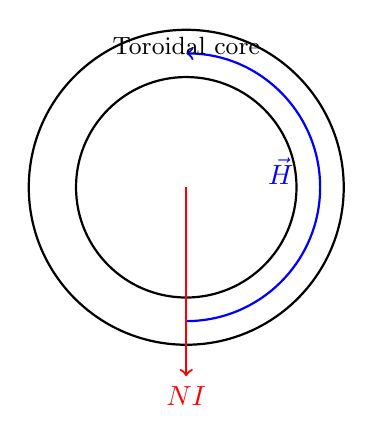
\begin{tikzpicture}
  \draw[thick] (0,0) circle(2);
  \draw[thick] (0,0) circle(1.4);
  \draw[->, thick, blue] (0,-1.7) arc(-90:90:1.7);
  \node[blue] at (1.2,0.2) {\( \vec{H} \)};
  \draw[->, red, thick] (0,0) -- (0,-2.4) node[below] {\( N I \)};
  \node at (0,1.8) {\small Toroidal core};
\end{tikzpicture}
\end{center}



\section*{Example 6-18: Magnetic Energy Stored in an Inductor}

\textbf{Problem:}  
An inductor with inductance \( L \) carries current \( I \). Find the magnetic energy stored and represent the circuit element.

\textbf{Solution:}

Magnetic energy stored is given by:
\[
W = \frac{1}{2} L I^2
\]

\begin{tcolorbox}
\[
\boxed{W = \frac{1}{2} L I^2}
\]
\end{tcolorbox}

\textbf{Diagram:}
\begin{center}
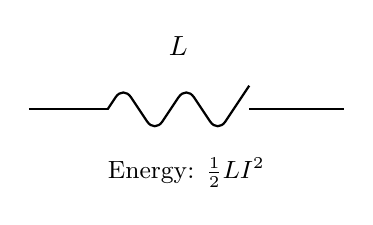
\begin{tikzpicture}
  \draw[thick] (0,0) -- (1,0);
  \draw[thick, rounded corners=5pt] (1,0) -- (1.2,0.3) -- (1.6,-0.3) -- (2,0.3) -- (2.4,-0.3) -- (2.8,0.3);
  \draw[thick] (2.8,0) -- (4,0);
  \node at (1.9,0.8) {\( L \)};
  \node at (2,-0.8) {\small Energy: \( \frac{1}{2} L I^2 \)};
\end{tikzpicture}
\end{center}



\section*{Example 6-19: Force on a Current Loop in a Magnetic Field}

\textbf{Problem:}  
A rectangular loop of current \( I \) lies in a uniform magnetic field \( \vec{B} \). Find the net force on the loop.

\textbf{Solution:}

The magnetic force on each segment:
\[
\vec{F} = I \vec{l} \times \vec{B}
\]

For opposite segments, forces cancel due to symmetry. So:
- Net force is zero in uniform field
- Torque may exist depending on orientation

\begin{tcolorbox}
\[
\boxed{\vec{F}_{\text{net}} = 0 \text{ (in uniform } \vec{B} \text{)}}
\]
\end{tcolorbox}

\textbf{Diagram:}
\begin{center}
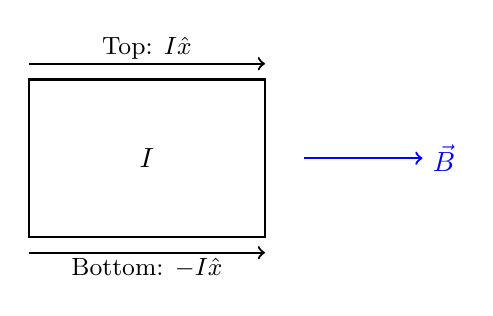
\begin{tikzpicture}
  \draw[thick] (0,0) rectangle (3,2);
  \draw[->, thick, blue] (3.5,1) -- (5,1) node[right] {\( \vec{B} \)};
  \node at (1.5,1) {\( I \)};
  \draw[->, thick] (0,2.2) -- (3,2.2);
  \node at (1.5,2.4) {\small Top: \( I \hat{x} \)};
  \draw[->, thick] (0,-0.2) -- (3,-0.2);
  \node at (1.5,-0.4) {\small Bottom: \( -I \hat{x} \)};
\end{tikzpicture}
\end{center}



\section*{Example 6-20: Torque on a Current Loop in a Magnetic Field}

\textbf{Problem:}  
A rectangular loop of area \( A \), carrying current \( I \), lies in a uniform magnetic field \( \vec{B} \). Find the torque acting on it.

\textbf{Solution:}

The magnetic dipole moment:
\[
\vec{m} = I \vec{A}
\]

Torque on the loop:
\[
\vec{\tau} = \vec{m} \times \vec{B}
\]

If loop is tilted at angle \( \theta \), magnitude of torque:
\[
\tau = I A B \sin\theta
\]

\begin{tcolorbox}
\[
\boxed{\vec{\tau} = \vec{m} \times \vec{B}}, \quad
\boxed{\tau = I A B \sin\theta}
\]
\end{tcolorbox}

\textbf{Diagram:}
\begin{center}
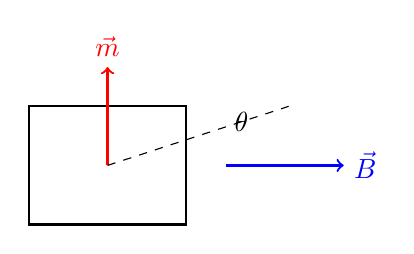
\begin{tikzpicture}
  \draw[thick] (0,0) -- (2,0) -- (2,1.5) -- (0,1.5) -- cycle;
  \draw[->, thick, blue] (2.5,0.75) -- (4,0.75) node[right] {\( \vec{B} \)};
  \draw[->, thick, red] (1,0.75) -- (1,2) node[above] {\( \vec{m} \)};
  \draw[dashed] (1,0.75) -- (3.3,1.5);
  \node at (2.7,1.3) {\( \theta \)};
\end{tikzpicture}
\end{center}



\section*{Example 6-21: Magnetic Boundary Conditions}

\textbf{Problem:}  
Two magnetic materials meet at a boundary with surface current density \( \vec{K}_s \). Determine the boundary conditions for \( \vec{B} \) and \( \vec{H} \).

\textbf{Solution:}

\textbf{Boundary Conditions:}
\[
\hat{n} \cdot (\vec{B}_2 - \vec{B}_1) = 0
\quad \text{(normal component of } \vec{B} \text{ continuous)}
\]
\[
\hat{n} \times (\vec{H}_2 - \vec{H}_1) = \vec{K}_s
\quad \text{(tangential component of } \vec{H} \text{ discontinuous)}
\]

\begin{tcolorbox}
\[
\boxed{
\begin{aligned}
\hat{n} \cdot (\vec{B}_2 - \vec{B}_1) &= 0 \\
\hat{n} \times (\vec{H}_2 - \vec{H}_1) &= \vec{K}_s
\end{aligned}
}
\]
\end{tcolorbox}

\textbf{Diagram:}
\begin{center}
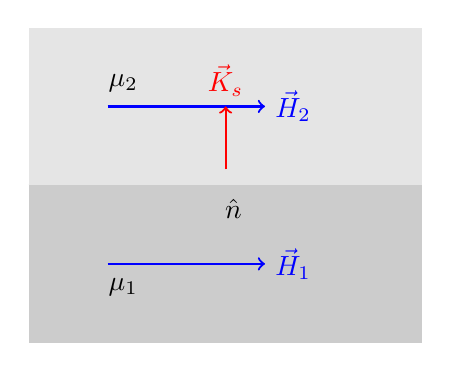
\begin{tikzpicture}
  \draw[thick] (0,0) -- (5,0);
  \fill[gray!20] (0,0) rectangle (5,2);
  \fill[gray!40] (0,0) rectangle (5,-2);
  \node at (1.2,1.3) {\( \mu_2 \)};
  \node at (1.2,-1.3) {\( \mu_1 \)};
  \draw[->, thick, blue] (1,1) -- (3,1) node[right] {\( \vec{H}_2 \)};
  \draw[->, thick, blue] (1,-1) -- (3,-1) node[right] {\( \vec{H}_1 \)};
  \draw[->, thick, red] (2.5,0.2) -- (2.5,1) node[above] {\( \vec{K}_s \)};
  \node at (2.6,-0.3) {\( \hat{n} \)};
\end{tikzpicture}
\end{center}



\section*{Example 6-22: Bound Currents in a Uniformly Magnetized Cylinder}

\textbf{Problem:}  
A long cylinder is uniformly magnetized along its axis with magnetization \( \vec{M} = M_0 \hat{z} \). Find the bound surface and volume currents.

\textbf{Solution:}

The bound volume current is:
\[
\vec{J}_b = \nabla \times \vec{M} = 0 \quad \text{(since } \vec{M} \text{ is constant)}
\]

The bound surface current is:
\[
\vec{K}_b = \vec{M} \times \hat{n} = M_0 \hat{z} \times \hat{r} = M_0 \hat{\phi}
\]

\begin{tcolorbox}
\[
\boxed{\vec{J}_b = 0}, \quad \boxed{\vec{K}_b = M_0 \hat{\phi}}
\]
\end{tcolorbox}

\textbf{Diagram:}
\begin{center}
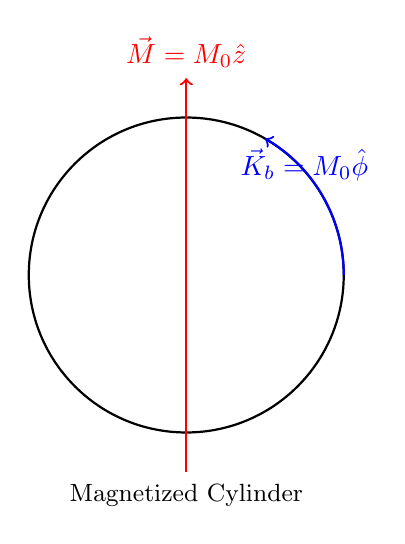
\begin{tikzpicture}
  \draw[thick] (0,0) circle(2);
  \draw[->, thick, red] (0,-2.5) -- (0,2.5) node[above] {\( \vec{M} = M_0 \hat{z} \)};
  \draw[->, thick, blue] (2,0) arc(0:60:2);
  \node[blue] at (1.5,1.4) {\( \vec{K}_b = M_0 \hat{\phi} \)};
  \node at (0,-2.8) {\small Magnetized Cylinder};
\end{tikzpicture}
\end{center}


\end{document}